\columnbreak
\section{Integration}
\subsection{Allgemeines}
Unter bi- oder multivariater Integration versteht man Integrale, welche sich über zwei oder mehr unabhängige Variablen erstrecken.
Sie haben die Form:
\[
    \int\limits_{\Omega} f(\omega) \diff \omega = \iint \cdots \int f(x_1, x_2, \ldots, x_n) \diff x_1 \diff x_2 \cdots \diff x_n
    \quad |\; \Omega \in \rreal^n
\]

\subsection{Normalbereiche}
Unter einem Normalbereich versteht man einen Bereich, welcher in allen Dimensionen so begrenzt ist, 
dass eine Funktion $f(x_1, x_2, \ldots, x_n)$ für jeden Eingangsvektor jeweils nur einen Funktionswert zurückgibt.


\example{Normalbereich in 2D}
% DONE: insert Normalbereich Image
\begin{center}
    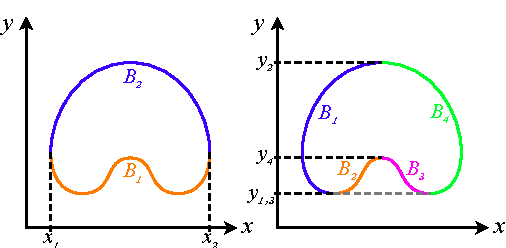
\includegraphics[width=0.8\columnwidth]{images/Normalbereiche_2D.pdf}
\end{center}
% TODO: add caption


\subsection{Satz von Fubini (Satz von Tonelli)}
Der Satz von Fubini besagt, dass die Reihenfolge der Integrationen vertauscht werden kann, sofern die Funktion integrierbar ist.

\[
    \iint\limits_{y_1 x_1}^{\; y_2 x_2} f(x,y)\diff x \diff y = \iint\limits_{x_1 y_1}^{\; x_2 y_2} f(x,y)\diff y \diff x%\iint f(x, y) \diff x \diff y = \int \left\lgroup \int f(x, y) \diff x \right\rgroup \diff y = \int \left\lgroup \int f(x, y) \diff y \right\rgroup \diff x
\]


\subsection{Erster Metrischer Tensor} % TODO: Vereinheitlichung d. Variablen und Funktionen
Der 1. metrische Tensor (oder auch \textbf{erste Fundamentalmatrix}, \textbf{erste Fundamentalform}, \textbf{metrische Grundform})
beschreibt den Zusammenhang zwischen einer Kurve oder Fläche im Parameterraum zum Raum, in dem sie sich befindet (z.B. 2D-Fläche im 3D-Raum).
Er besteht aus den Skalarprodukten der partiellen Ableitungsvektoren nach den Parametern.
\[
    g_{ij} = \frac{\partial \vec{S}}{\partial u_i} \dotp \frac{\partial \vec{S}}{\partial u_j}
\]
Folglich ergibt sich die Matrix: $\begin{pmatrix}
    E & F\\
    F & G
\end{pmatrix} = \begin{pmatrix}
    g_{11} & g_{12}\\
    g_{21} & g_{22}
\end{pmatrix}$

Die Einträge dieser Matrix werden benötigt, um Längen- oder Flächen(elemente) zu berechnen.

% TODO: subsubsection Flächen-, Längen- & Winkelerhaltung (Siehe Moodle Woche 11)

\example{Längenberechnung}
Eine Flächenkurve sei als $\vec{x}(t) = \begin{pmatrix}
    u(t)\\
    v(t)
\end{pmatrix}$ gegeben.
Davon wird das totale Differential gebildet: 
\[
    \dot{\vec{x}} = \vec{x}_u \cdot \dot{u} + \vec{x}_v \cdot \dot{v}
\]
Um die Länge des Vektors (Längenelement) zu erhalten, muss man diesen im ersten Schritt quadrieren:
\[
    (\dot{\vec{x}})^2 = g_{11} \dot{u}^2 + 2 g_{12} \dot{u} \dot{v} + g_{22} \dot{v}^2
\]
Das einzelne Längenelement ist somit:
\[
    \diff s = \sqrt{g_{11} \diff u^2 + 2 g_{12} \diff u \diff v + g_{22} \diff v^2}
\]
Summiert man nun alle $\diff s$ über die Kurve, so ergibt dies das Integral für die gesamte Länge:
\[
    s = \int\limits_{a}^{b} \sqrt{g_{11} \dot{u}^2 + 2 g_{12} \dot{u} \dot{v} + g_{22} \dot{v}^2} \diff t
\]


\example{Flächenberechnung}
Es sei eine parametrisierte Fläche als Funktion $\vec{S}(u,v) = \begin{pmatrix}
    x(u,v)\\
    y(u,v)\\
    z(u,v)
\end{pmatrix}$ gegeben.
Das Flächenelement lässt sich aus einem Parallelogramm der beiden partiellen Ableitungsvektoren bilden, 
was dem Betrag des Kreuzproduktes bzw. der Determinante entspricht:
\[
    \diff S = \sqrt{\abs{\det\abs{g_{ij}}}}\diff u \diff v = \sqrt{g_{11}g_{22} - g_{12}^2} \diff u \diff v = \abs{\frac{\partial \vec{S}}{\partial u} \times \frac{\partial \vec{S}}{\partial v}} \diff u \diff v
\]
Daraus ergibt sich die Fläche über das Doppelintegral:
\[
    S = \iint\limits_{v_1\, u_1}^{v_2\, u_2} \sqrt{g_{11}g_{22} - g_{12}^2} \diff u \diff v
\]


% DONE: Längenintegrale (3D)
% TODO: Längenintegrale (2D)
\subsection{Längenintegrale}
\subsubsection{Längenelemente}\label{section:int_multivar:längenelemente}
$$
 \diff s^2 
    = \underbrace{\diff x^2 + \diff y^2 + \diff z^2}_{\text{Kartesisch}}
    = \underbrace{\diff r^2 + r^2 \diff \varphi^2 + \diff z^2}_{\text{Zylindrisch}}
    = \underbrace{\diff r^2 + r^2 \diff \theta^2 + r^2 \sin^2 \theta \diff \phi^2}_{\text{Sphärisch}}
$$
\subsubsection{Länge einer Funktion}
Die Bestimmung der Länge einer Kurve kann in folgende Schritte unterteilt werden:
\begin{enumerate}
    \item \myul{\textbf{Funktion in die Parameterdarstellung überführen (sofern nicht gegeben):}}
    \item[] Dafür wird einer der Parameter (z.B. $x$ oder $\theta$) $=t$ gesetzt und die anderen Parameter ebenfalls als Funktion von $t$ ausgedrückt.
    \item \myul{\textbf{Integral aufstellen:}}
    \item[] Das Integral in der Form $ \iiint \diff s $ wird mit $\frac{\diff t}{\diff t}$ erweitert.
    \item \myul{\textbf{Das Integral lösen}}
\end{enumerate}

% \subsubsection{Beispiel}
\example{Längenintegral in kartesischen Koordinaten}
Es soll die Länge der Kurve $\vec{v}(t) = \begin{pmatrix}x(t)\\y(t)\\z(t)\end{pmatrix}$ auf dem Interval $[t_1, t_2]$ bestimmt werden.
Dazu werden die oben genannten Schritte abgearbeitet:
\begin{enumerate}
    \item \textbf{Funktion in die Parameterdarstellung überführen}
    \item[] Hier nicht nötig. % evtl. TODO: Beispiel wählen, bei dem das nötig ist.
    \item \textbf{Integral aufstellen} 
    \item[] $ \iiint \diff s = \iiint \sqrt{\diff x^2 + \diff y^2 + \diff z^2} = \int_{t_1}^{t_2} \sqrt{\left(\frac{\diff x}{\diff t}\right)^2 + \left(\frac{\diff y}{\diff t}\right)^2 + \left(\frac{\diff z}{\diff t}\right)^2} \diff t$
    \item Integral lösen
    \item[] $\frac{\diff x}{\diff t}$, $\frac{\diff y}{\diff t}$ und $\frac{\diff z}{\diff t}$ ausrechnen, einsetzen, integrieren.
\end{enumerate}


% DONE: Flächenintegrale (2D, 3D)
\subsection{(Ober-)Flächenintegrale}
\subsubsection{Flächenelemente}
% TODO: stimmt das?
Das Bestimmen der Flächenelemente ist in drei Dimensionen nicht wie bei den Längen- und Volumenelementen pauschal möglich.
Dies, da jeweils nur über zwei der drei Koordinaten integriert werden muss.
Ein einfaches Verfahren für das Berechnen von Flächeninhalten schafft jedoch abhilfe.
\subsubsection{Flächeninhalt einer Oberfläche}
Für das Berechnen der Oberflächen von Funktionen des Typs $f(a, b)$ in 3D kann die Formel
$$ S = \int\limits_{B} \int\limits_{A} \sqrt{(f_{a})^2 + (f_{b})^2 + 1} \diff a \diff b $$
verwendet werden. Dabei repräsentieren $a$ und $b$ die beiden Koordinatenrichtungen, in denen sich die Fläche erstreckt.
$f_a$ und $f_b$ sind die partiellen Ableitungen der Funktion $f(a, b)$ nach $a$ bzw. $b$.
\medskip

\myul{\bf{Beispiele zur Veranschaulichung:}}\\
Es soll die Oberfläche der Funktion $ f(x, y) $ im Bereich $ x \in [x_1, x_2], y \in [y_1, y-2] $ bestimmt werden.
Das entsprechende integral lautet:
$$ S = \int_{y_1}^{y_2} \int_{x_1}^{x_2} \sqrt{(f_{x})^2 + (f_{y})^2 + 1} \diff x \diff y $$

Wäre die Funktion $f$ stat in kartesischen in polaren oder sphärischen Koordinaten formuliert, ändern sich lediglich die Namen der Variablen. 
Folglich ist das zu einer in sphärischen Koordinaten definierten Fkt. $f(\theta, \phi)$ gehörende Integral
$$ S = \int_{\phi_1}^{\phi_2} \int_{\theta_1}^{\theta_2} \sqrt{(f_{\theta})^2 + (f_{\phi})^2 + 1} \diff \theta \diff \phi $$
sehr leicht aufzustellen.


\subsubsection{Allgemeine Wendelfläche}
Die allgemeine Wendelfläche rotiert und verschiebt eine parametrisierte 3D Kurve $\vec{r}(t) = (x(t), y(t), z(t))\tr$ im Raum.

Parametrisierung bei vertikaler Rotationsachse und vertikaler Verschiebungsrichtung ($z$-Achse):
\[
    \vec{S}(t, \varphi) = \begin{pmatrix}
        \begin{pmatrix}
            \cos(\varphi) & -\sin(\varphi)\\
            \sin(\varphi) & \cos(\varphi)
        \end{pmatrix}
        \cdot \begin{pmatrix}
            x(t)\\
            y(t)
        \end{pmatrix}\\
        z(t) + c \cdot \varphi
    \end{pmatrix}
    \quad (t_1 \leq t \leq t_2, \land \varphi \in \rreal\;, c \equiv const.)
\]

Bei $c = 1$ \textrightarrow\ Voller Meter bei einer Kurve % TODO: Check this



% TODO: Volumenintegrale (3D)
\subsection{Volumenintegrale}
\subsubsection{Volumenelemente}
$$ 
 \diff V 
    = \underbrace{\diff x \diff y \diff z}_{\text{Kartesisch}}
    = \underbrace{r \diff r \diff \varphi \diff z}_{\text{Zylindrisch}}
    = \underbrace{r^2 \sin \theta \diff \theta \diff \phi \diff r}_{\text{Sphärisch}}
$$


% TODO: Andwendungsformeln
% \subsection{Anwendungsformeln}
% TODO: Anwendungsformeln 2D (Doppelintegrale)
\subsection{Anwendungsformeln 2D (Doppelintegrale)}
\resizebox{\linewidth}{!}{
    \begin{tabular}{|l|l|l|}
        \hline
        \bf{Allgemein} & \bf{Kartesische Koordinaten} & \bf{Polarkoordinaten} \\
        \hline

        \multicolumn{3}{|l|}{\bf{Flächeninhalt einer ebenen Figur $F$}} \\\hline
        $ A = \iint\limits_{F} \diff F $ & 
        $ = \int\limits_{X}\int\limits_{Y} \diff y \diff x $ &
        $ = \int\limits_{\Phi}\int\limits_{R} r \diff r \diff \varphi $ \\\hline

        \multicolumn{3}{|l|}{\bf{Oberfläche einer Ebene in drei Dimensionen}} \\\hline
        % TODO: Evtl. umschreiben, dass man es besser versteht...
        $ S = \iint\limits_{A} \frac{1}{\cos \gamma} \diff A $ & 
        $ = \int\limits_{X}\int\limits_{Y} \sqrt{1 + \left(\frac{\partial z}{\partial x}\right)^2 + \left(\frac{\partial z}{\partial y}\right)^2} \diff y \diff x $ &
        $ = \int\limits_{\Phi}\int\limits_{R} \sqrt{r^2 + r^2\left(\frac{\partial z}{\partial r}\right)^2 + \left(\frac{\partial z}{\partial \varphi}\right)^2} \diff r \diff \varphi $ \\\hline
        
        \multicolumn{3}{|l|}{\bf{Volumen eines Zylinders}} \\\hline
        $ V = \iint\limits_{A} z \diff A $ & 
        $ = \int\limits_{X}\int\limits_{Y} z \diff y \diff x $ &
        $ = \int\limits_{\Phi}\int\limits_{R} z r \diff r \diff \varphi $ \\\hline

        \multicolumn{3}{|l|}{\bf{Trägheitsmoment einer ebenen Figur $F$, bezogen auf die x-Achse}} \\\hline
        $ I_x = \iint\limits_{F} y^2 \diff F $ & 
        $ = \int\limits_{X}\int\limits_{Y} (y^2) \diff y \diff x $ &
        $ = \int\limits_{\Phi}\int\limits_{R} (r^2 \sin^2\varphi) r \diff r \diff \varphi $ \\\hline

        \multicolumn{3}{|l|}{\bf{Trägheitsmoment einer ebenen Figur $F$, bezogen auf den Pol $(0, 0)$}} \\\hline
        $ I_x = \iint\limits_{F} r^2 \diff F $ & 
        $ = \int\limits_{X}\int\limits_{Y} (x^2 + y^2) \diff y \diff x $ &
        $ = \int\limits_{\Phi}\int\limits_{R} (r^2) r \diff r \diff \varphi $ \\\hline

        \multicolumn{3}{|l|}{\bf{Masse einer ebenen Figur $F$ mit Dichtefunktion $\varrho$}} \\\hline
        $ m = \iint\limits_{F} \varrho \diff F $ & 
        $ = \int\limits_{X}\int\limits_{Y} \varrho (x, y) \diff y \diff x $ &
        $ = \int\limits_{\Phi}\int\limits_{R} \varrho (r, \varphi) r \diff r \diff \varphi $ \\\hline

        \multicolumn{3}{|l|}{\bf{Koordinaten des Schwerpunkts $S$ einer homogenen, ebenen Figur $F$}} \\\hline
        $ x_{S} = \frac{\iint\limits_{F} x \diff F}{A} $ & 
        $ = \frac{\int\limits_{X}\int\limits_{Y} x \diff y \diff x}{\int\limits_{X}\int\limits_{Y} \diff y \diff x} $ &
        $ = \frac{\int\limits_{\Phi}\int\limits_{R} r^2 \cos \varphi \diff r \diff \varphi}{\int\limits_{\Phi}\int\limits_{R} r \diff r \diff \varphi} $ \\
        $ y_{S} = \frac{\iint\limits_{F} y \diff F}{A} $ & 
        $ = \frac{\int\limits_{X}\int\limits_{Y} y \diff y \diff x}{\int\limits_{X}\int\limits_{Y} \diff y \diff x} $ &
        $ = \frac{\int\limits_{\Phi}\int\limits_{R} r^2 \sin \varphi \diff r \diff \varphi}{\int\limits_{\Phi}\int\limits_{R} r \diff r \diff \varphi} $ \\\hline
    \end{tabular}
}

\smallskip
Hinweis: Damit die Flächenelemente leichter erkennbar und die Formeln entsprechend besser nachvollziebar sind, wurden sie teilweise nicht vollständig vereinfacht.


% TODO: Anwendungsformeln 3D (Dreifachintegrale)
\subsection{Anwendungsformeln 3D (Dreifachintegrale)}
\resizebox{\linewidth}{!}{
    \begin{tabular}{|l|l|l|l|}  
        \hline
        \bf{Allgemein} & \bf{Kartesische Koordinaten} & \bf{Zylinderkoordinaten} & \bf{Kugelkoordinaten} \\
        \hline
        \multicolumn{4}{|l|}{\bf{Volumen eines Körpers $K$}} \\
        \hline
        $ V = \iiint\limits_{K} \diff V $ & 
        $ = \iiint \diff x \diff y \diff z $ &
        $ = \iiint r \diff r \diff \phi \diff z $ &
        $ = \iiint r^2 \sin \theta \diff \theta \diff \phi \diff r $ \\
        \hline

        \multicolumn{4}{|l|}{\bf{Trägheitsmoment eines Körpers $K$, bezogen auf die Z-Achse}} \\
        \hline
        $ I_z = \iiint\limits_{K} r^2 \diff V $ & 
        $ = \iiint (x^2 + y^2) \diff x \diff y \diff z $ &
        $ = \iiint (r^2) r \diff r \diff \phi \diff z $ &
        $ = \iiint (r^2 \sin^2 \theta) r^2 sin \theta \diff \theta \diff \phi \diff r $ \\
        \hline

        \multicolumn{4}{|l|}{\bf{Masse eines Körpers $K$ mit der Dichtefunktion $\varrho$}} \\
        \hline
        $ M = \iiint\limits_{K} \varrho \diff V $ & 
        $ = \iiint \varrho (x, y, z) \diff x \diff y \diff z $ &
        $ = \iiint \varrho (r, \phi, z) r \diff r \diff \phi \diff z $ &
        $ = \iiint \varrho (r, \theta, \phi) r^2 sin \theta \diff \theta \diff \phi \diff r $ \\
        \hline

        \multicolumn{4}{|l|}{\bf{Koordinaten des Schwerpunktes $S$ eines homogenen Körpers $K$}} \\
        \hline
        $ x_{S} = \frac{\iiint\limits_{K} x \diff V}{V} $ & 
        $ = \frac{\iiint (x) \diff x \diff y \diff z}{V} $ &
        $ = \frac{\iiint (r \cos \phi) r \diff r \diff \phi \diff z}{V} $ &
        $ = \frac{\iiint (r \sin \theta \cos \phi) r^2 sin \theta \diff \theta \diff \phi \diff r}{V} $ \\

        $ y_{S} = \frac{\iiint\limits_{K} y \diff V}{V} $ & 
        $ = \frac{\iiint (y) \diff x \diff y \diff z}{V} $ &
        $ = \frac{\iiint (r \sin \phi) r \diff r \diff \phi \diff z}{V} $ &
        $ = \frac{\iiint (r \sin \theta \sin \phi) r^2 sin \theta \diff \theta \diff \phi \diff r}{V} $ \\

        $ z_{S} = \frac{\iiint\limits_{K} z \diff V}{V} $ & 
        $ = \frac{\iiint (z) \diff x \diff y \diff z}{V} $ &
        $ = \frac{\iiint (z) r \diff r \diff \phi \diff z}{V} $ &
        $ = \frac{\iiint (r \cos \theta) r^2 sin \theta \diff \theta \diff \phi \diff r}{V} $ \\
        \hline
    \end{tabular}
}

\smallskip
Hinweis: Damit die Volumenelemente leichter erkennbar und die Formeln entsprechend besser nachvollziebar sind, wurden sie teilweise nicht vollständig vereinfacht.


% \subsection{Umrechnungen}
% \subsubsection{Kartesische Koordinaten $\leftrightarrow$ Polarkoordinaten}

% \subsection{Anwendungsformeln}
% \resizebox{\linewidth}{!}{
%     \begin{tabular}{|l|l|l|}
%         \hline
%         \bf{Allgemein} & \bf{Kartesische Koordinaten} & \bf{Polarkoordinaten} \\
%         \hline

%         \multicolumn{3}{|l|}{\bf{Flächeninhalt einer ebenen Figur $F$}} \\\hline
%         $ A = \iint\limits_{F} \diff a $ & 
%         $ = \int\limits_{X}\int\limits_{Y} \diff y \diff x $ &
%         $ = \int\limits_{\Phi}\int\limits_{R} r \diff r \diff \varphi $ \\\hline

%         \multicolumn{3}{|l|}{\bf{Oberfläche einer Ebene in drei Dimensionen}} \\\hline
%         % TODO: Evtl. umschreiben, dass man es besser versteht...
%         $ S = \iint\limits_{A} \frac{1}{\cos \gamma} \diff a $ & 
%         $ = \int\limits_{X}\int\limits_{Y} \sqrt{1 + \left(\frac{\partial z}{\partial x}\right)^2 + \left(\frac{\partial z}{\partial y}\right)^2} \diff y \diff x $ &
%         $ = \int\limits_{\Phi}\int\limits_{R} \sqrt{r^2 + r^2\left(\frac{\partial z}{\partial r}\right)^2 + \left(\frac{\partial z}{\partial \varphi}\right)^2} \diff r \diff \varphi $ \\\hline
        
%         \multicolumn{3}{|l|}{\bf{Volumen eines Zylinders}} \\\hline
%         $ V = \iint\limits_{A} z \diff a $ & 
%         $ = \int\limits_{X}\int\limits_{Y} z \diff y \diff x $ &
%         $ = \int\limits_{\Phi}\int\limits_{R} z r \diff r \diff \varphi $ \\\hline

%         \multicolumn{3}{|l|}{\bf{Trägheitsmoment einer ebenen Figur $F$, bezogen auf die x-Achse}} \\\hline
%         $ I_x = \iint\limits_{F} y^2 \diff a $ & 
%         $ = \int\limits_{X}\int\limits_{Y} (y^2) \diff y \diff x $ &
%         $ = \int\limits_{\Phi}\int\limits_{R} (r^2 \sin^2\varphi) r \diff r \diff \varphi $ \\\hline

%         \multicolumn{3}{|l|}{\bf{Trägheitsmoment einer ebenen Figur $F$, bezogen auf den Pol $(0, 0)$}} \\\hline
%         $ I_x = \iint\limits_{F} r^2 \diff a $ & 
%         $ = \int\limits_{X}\int\limits_{Y} (x^2 + y^2) \diff y \diff x $ &
%         $ = \int\limits_{\Phi}\int\limits_{R} (r^2) r \diff r \diff \varphi $ \\\hline

%         \multicolumn{3}{|l|}{\bf{Masse einer ebenen Figur $F$ mit Dichtefunktion $\varrho$}} \\\hline
%         $ m = \iint\limits_{F} \varrho \diff a $ & 
%         $ = \int\limits_{X}\int\limits_{Y} \varrho (x, y) \diff y \diff x $ &
%         $ = \int\limits_{\Phi}\int\limits_{R} \varrho (r, \varphi) r \diff r \diff \varphi $ \\\hline

%         \multicolumn{3}{|l|}{\bf{Koordinaten des Schwerpunkts $S$ einer homogenen, ebenen Figur $F$}} \\\hline
%         $ x_{S} = \frac{\iint\limits_{F} x \diff a}{A} $ & 
%         $ = \frac{\int\limits_{X}\int\limits_{Y} x \diff y \diff x}{\int\limits_{X}\int\limits_{Y} \diff y \diff x} $ &
%         $ = \frac{\int\limits_{\Phi}\int\limits_{R} r^2 \cos \varphi \diff r \diff \varphi}{\int\limits_{\Phi}\int\limits_{R} r \diff r \diff \varphi} $ \\
%         $ y_{S} = \frac{\iint\limits_{F} y \diff a}{A} $ & 
%         $ = \frac{\int\limits_{X}\int\limits_{Y} y \diff y \diff x}{\int\limits_{X}\int\limits_{Y} \diff y \diff x} $ &
%         $ = \frac{\int\limits_{\Phi}\int\limits_{R} r^2 \sin \varphi \diff r \diff \varphi}{\int\limits_{\Phi}\int\limits_{R} r \diff r \diff \varphi} $ \\\hline
%     \end{tabular}
% }

% \resizebox{\linewidth}{!}{
%     \begin{tabular}{|l|l|l|l|}  
%         \hline
%         \bf{Allgemein} & \bf{Kartesische Koordinaten} & \bf{Zylinderkoordinaten} & \bf{Kugelkoordinaten} \\
%         \hline
%         \multicolumn{4}{|l|}{\bf{Volumen eines Körpers $K$}} \\
%         \hline
%         $ V = \iiint\limits_{K} \diff V $ & 
%         $ = \iiint \diff x \diff y \diff z $ &
%         $ = \iiint r \diff r \diff \phi \diff z $ &
%         $ = \iiint r^2 \sin \theta \diff \theta \diff \phi \diff r $ \\
%         \hline

%         \multicolumn{4}{|l|}{\bf{Trägheitsmoment eines Körpers $K$, bezogen auf die Z-Achse}} \\
%         \hline
%         $ I_z = \iiint\limits_{K} r^2 \diff V $ & 
%         $ = \iiint (x^2 + y^2) \diff x \diff y \diff z $ &
%         $ = \iiint (r^2) r \diff r \diff \phi \diff z $ &
%         $ = \iiint (r^2 \sin^2 \theta) r^2 sin \theta \diff \theta \diff \phi \diff r $ \\
%         \hline

%         \multicolumn{4}{|l|}{\bf{Masse eines Körpers $K$ mit der Dichtefunktion $\varrho$}} \\
%         \hline
%         $ M = \iiint\limits_{K} \varrho \diff V $ & 
%         $ = \iiint \varrho (x, y, z) \diff x \diff y \diff z $ &
%         $ = \iiint \varrho (r, \phi, z) r \diff r \diff \phi \diff z $ &
%         $ = \iiint \varrho (r, \theta, \phi) r^2 sin \theta \diff \theta \diff \phi \diff r $ \\
%         \hline

%         \multicolumn{4}{|l|}{\bf{Koordinaten des Schwerpunktes $S$ eines homogenen Körpers $K$}} \\
%         \hline
%         $ x_{S} = \frac{\iiint\limits_{K} x \diff V}{V} $ & 
%         $ = \frac{\iiint (x) \diff x \diff y \diff z}{V} $ &
%         $ = \frac{\iiint (r \cos \phi) r \diff r \diff \phi \diff z}{V} $ &
%         $ = \frac{\iiint (r \sin \theta \cos \phi) r^2 sin \theta \diff \theta \diff \phi \diff r}{V} $ \\

%         $ y_{S} = \frac{\iiint\limits_{K} y \diff V}{V} $ & 
%         $ = \frac{\iiint (y) \diff x \diff y \diff z}{V} $ &
%         $ = \frac{\iiint (r \sin \phi) r \diff r \diff \phi \diff z}{V} $ &
%         $ = \frac{\iiint (r \sin \theta \sin \phi) r^2 sin \theta \diff \theta \diff \phi \diff r}{V} $ \\

%         $ z_{S} = \frac{\iiint\limits_{K} z \diff V}{V} $ & 
%         $ = \frac{\iiint (z) \diff x \diff y \diff z}{V} $ &
%         $ = \frac{\iiint (z) r \diff r \diff \phi \diff z}{V} $ &
%         $ = \frac{\iiint (r \cos \theta) r^2 sin \theta \diff \theta \diff \phi \diff r}{V} $ \\
%         \hline
%     \end{tabular}
% }



% \section{Koordinatensysteme}
% \subsection{2D Koordinatensysteme}
% Neben den Kartesischen Koordinatensystemen kommen in zweidimensionalen Räumen auch Polare Koordinatensysteme zum Einsatz.
% Die beiden Systeme können mit Hilfe der Trigonometrie in einander überführt werden.

% \subsubsection{Umrechnung Kartesisch $\leftrightarrow$ Polar}
% \begin{minipage}{0.29\linewidth}
%     \myul{Polar zu Kartesisch}
%     \[
%     \begin{pmatrix}
%         x \\
%         y
%     \end{pmatrix}
%     =
%     \begin{pmatrix}
%         r \cdot \cos{\varphi}\\
%         r \cdot \sin{\varphi}
%     \end{pmatrix}
%     \]
% \end{minipage}
% \hfill
% \begin{minipage}{0.29\linewidth}
%     \myul{Kartesisch zu Polar}
%     \[
%     \begin{pmatrix}
%         r \\
%         \varphi
%     \end{pmatrix}
%     =
%     \begin{pmatrix}
%         \sqrt{x^2+y^2}\\
%         \tan^{-1}{\frac{y}{x}}
%     \end{pmatrix}
%     \]
% \end{minipage}
% \hfill
% \begin{minipage}{0.29\linewidth}
%     \begin{center}
%         \begin{tikzpicture} [scale = 1.5]
%             % Kartesische Achsen
%             \draw[-{latex}] (0, 0) -- (1, 0) node [below] {$x$} ;
%             \draw[-{latex}] (0, 0) -- (0, 1) node [left]  {$y$} ;

%             % Punkt p
%             \fill (0.5, 0.8) circle (1pt) node [anchor=south west] {$\vec{p}$};

%             % Länge r
%             \draw (0, 0) -- (0.5, 0.8) node [midway, above left] {$r$};
%             % Winkel phi
%             \draw [-{latex}] (0.5, 0) arc (0:58:0.5) node [midway, right] {$\varphi$};
%         \end{tikzpicture}
%     \end{center}
% \end{minipage}

% Dabei ist zu beachten, dass $\tan^{-1}$ nur werte von $-\frac{\pi}{2}$ bis $\frac{\pi}{2}$ liefert, für $\varphi$ jedoch $\varphi \in [0, \pi]$ gelten soll. 
% $\varphi$ wird also, je nach dem in welchem Quadranten sich $\vec{p}$ befindet, nach folgendem Schema berechnet:
% \begin{center}
%     \begin{tikzpicture}
%         % Achsen 
%         \draw [-{latex}] (-2, 0) -- (2, 0) node [below] {$x$};
%         \draw [-{latex}] (0, -0.8) -- (0, 0.8) node [left] {$y$};
%         % Formeln
%         \node at ( 1,  0.4) {$       \tan^{-1}\frac{y}{x}$};
%         \node at ( 1, -0.4) {$2\pi + \tan^{-1}\frac{y}{x}$};
%         \node at (-1, -0.4) {$\pi  + \tan^{-1}\frac{y}{x}$};
%         \node at (-1,  0.4) {$\pi  + \tan^{-1}\frac{y}{x}$};
%     \end{tikzpicture}
% \end{center}

% Um eine ganzes Integral vom einen Koordinatensystem ins andere zu überführen, muss zum einen die Funktion $ f(x, y) $ zu $ f(r, \varphi) $ (oder umgekehrt) umgeschrieben, sowie die differentiale angepasst werden.
% Hier dafür einige gängige Elemente:

% \begin{tabular}{l c c}
%                          & \bf{Kartesisch}                   & \bf{Polar}                                                       \\
%     \bf{x-Achsenelement} & $\diff x$                         & $\diff x = \cos \varphi \diff r - r \sin \varphi \diff \varphi$  \\
%     \bf{y-Achsenelement} & $\diff y$                         & $\diff x = \sin \varphi \diff r + r \cos \varphi \diff \varphi$  \\
%     \bf{Linienelement  } & $\diff s^2 = \diff x^2 \diff y^2$ & $\diff s^2 = \diff r^2 + r^2 \diff \varphi^2$                    \\
%     \bf{Flächenelement } & $\diff A = \diff x \diff y$       & $\diff A = r \diff r \diff \varphi$                              \\
% \end{tabular}

% % \subsection{2D Transformation Polar zu Kartesisch}
% % TODO: Das isch ja ds gliiche wie obe beschribe, oder?
% %       Wänn da no meh ane sött wüsstich nöd was... -Flurin
% % T $=$ Transformation
% % \[
% %     \text{Polar } (r,\varphi) \xrightarrow{T} (x,y) \text{ Kartesisch}
% % \]

% % \[
% % \begin{pmatrix}
% %     x=r\cdot\cos(\varphi) \text{ } \cor{\mathbb{R}} \\
% %     y=r\cdot\sin(\varphi) \text{ } \cor{\mathbb{R}} 
% % \end{pmatrix}
% % \text{2D}
% % \]

% % Die Funktionen für $x$ und $y$ sind skalare Funktion.

% %     \begin{ctabular}{ll}
% %         $x=x(r;\varphi)$ & $ y=y(r;\varphi)$
% %     \end{ctabular}


% \subsection{3D Koordinatensysteme}
% \resizebox{\linewidth}{!}{
%     \begin{tabular}{c c c}
%         \myul{\textbf{Kartesisch}} & \myul{\textbf{Zylindrisch}} & \myul{\textbf{Sphärisch}} \\
        
%         \tdplotsetmaincoords{70}{110}
%         \begin{tikzpicture}[baseline=(current bounding box.north), tdplot_main_coords, scale=2]
%             % Koordinatensystem
%             \draw [-{latex}] (0, 0, 0) -- (1, 0, 0) node [below left] {$x$};
%             \draw [-{latex}] (0, 0, 0) -- (0, 1, 0) node [right]      {$y$};
%             \draw [-{latex}] (0, 0, 0) -- (0, 0, 1) node [right]      {$z$};
%             % Punkt bei (0.75,0.75,0.75)
%             \fill (0.75, 0.75, 0.75) circle (1pt) node [above right] {$P(x, y, z)$};
%             % Koordinatenkomponenten
%             \draw [dashed] (0, 0.75, 0)    -- (0.75, 0.75, 0)    node [midway, below right] {$x$};
%             \draw [dashed] (0.75, 0, 0)    -- (0.75, 0.75, 0)    node [midway, below left]  {$y$};
%             \draw [dashed] (0.75, 0.75, 0) -- (0.75, 0.75, 0.75) node [midway, right]       {$z$};
%         \end{tikzpicture} &

%         \tdplotsetmaincoords{70}{110}
%         \begin{tikzpicture}[baseline=(current bounding box.north), tdplot_main_coords, scale=2]
%             % Koordinatensystem
%             \draw [-{latex}] (0, 0, 0) -- (1, 0, 0) node [below left] {$x$};
%             \draw [-{latex}] (0, 0, 0) -- (0, 1, 0) node [right]      {$y$};
%             \draw [-{latex}] (0, 0, 0) -- (0, 0, 1) node [right]      {$z$};
%             % Punkt bei (0.75,0.75,0.75)
%             \fill (0.75, 0.75, 0.75) circle (1pt) node [above right] {$P(r_{\rm z}, \varphi, z)$};
%             % Koordinatenkomponenten
%             \draw [dashed] (0,0,0)         --  (0.75, 0.75, 0)    node [midway, above right, inner sep=0pt] {$r_{\rm z}$};
%             \draw [-{latex}]     (0.5,0,0)       arc (0:45:0.5)         node [midway, below]       {$\varphi$};
%             \draw [dashed] (0.75, 0.75, 0) --  (0.75, 0.75, 0.75) node [midway, right]       {$z$};
%         \end{tikzpicture} &

%         \tdplotsetmaincoords{70}{110}
%         \begin{tikzpicture}[baseline=(current bounding box.north), tdplot_main_coords, scale=2]
%             % Koordinatensystem
%             \draw [-{latex}] (0, 0, 0) -- (1, 0, 0) node [below left] {$x$};
%             \draw [-{latex}] (0, 0, 0) -- (0, 1, 0) node [right]      {$y$};
%             \draw [-{latex}] (0, 0, 0) -- (0, 0, 1) node [right]      {$z$};
%             % Punkt bei (0.75,0.75,0.75)
%             \fill (0.75, 0.75, 0.75) circle (1pt) node [above right] {$P(r_{\rm s}, \theta, \phi)$};
%             % Koordinatenkomponenten
%             \draw [dotted] (0,0,0) -- (0.75, 0.75, 0) -- (0.75, 0.75, 0.75);
%             \draw [-{latex}]     (0.5,0,0) arc (0:45:0.5)         node [midway, below]       {$\phi$};
%             \draw [dashed] (0, 0, 0) --  (0.75, 0.75, 0.75) node [midway, below right] {$r_{\rm s}$};
%             \tdplotsetthetaplanecoords {90}
%             \tdplotdrawarc [tdplot_rotated_coords, -{latex}] {(0, 0, 0)} {0.5} {0} {45} {anchor=south} {$\theta$}
%         \end{tikzpicture} \\

%         $ 
%         \begin{pmatrix}
%             x \\ y \\ z
%         \end{pmatrix} 
%         =
%         \begin{pmatrix}
%             r \cos \varphi \\ r \sin \varphi \\ z
%         \end{pmatrix}
%         =
%         \begin{pmatrix}
%             r \sin \theta \cos \phi \\ r \sin \theta \sin \phi \\ r \cos \theta
%         \end{pmatrix}
%         $ &
%         $ 
%         \begin{pmatrix}
%             r_{\rm z} \\ \varphi \\ z
%         \end{pmatrix} 
%         =
%         \begin{pmatrix}
%             \sqrt{x^2 + y^2} \\ \tan^{-1}\frac{y}{x} \\ z
%         \end{pmatrix}
%         =
%         \begin{pmatrix}
%             r_{\rm s} \sin \theta \\ \phi \\ r_{\rm s} \cos \theta
%         \end{pmatrix}
%         $ &
%         $ 
%         \begin{pmatrix}
%             r_{\rm s} \\ \theta \\ \phi
%         \end{pmatrix} 
%         =
%         \begin{pmatrix}
%             \sqrt{x^2+y^2+z^2} \\ \cos^{-1} \frac{z}{\sqrt{x^2+y^2+z^2}} \\ \sgn(y) \cos^{-1} \frac{x}{\sqrt{x^2+y^2}}
%         \end{pmatrix}
%         =
%         \begin{pmatrix}
%             \sqrt{r_{\rm z}^2+z^2} \\ \tan^{-1}\frac{r_{\rm z}}{z} \\ \varphi
%         \end{pmatrix}
%         $ \\
%     \end{tabular}
% }
% \smallskip
% \subsubsection{Umrechnen zwischen Koordinatensystemen}
% Beim Umrechnen zwischen den Koordinatensystemen gelten im Grunde genommen die obigen Formeln. 
% Dabei muss jedoch in einigen Fällen auf die Wertebereiche von den trigonometrischen Funktionen rücksicht genommen werden.

% \myul{\textbf{Zylindrisch $\rightarrow$ Kartesisch:}}\\
% \myul{\textbf{Sphärisch $\rightarrow$ Kartesisch:}}\\
% Keine weiteren Berücksichtigungen nötig, die Berechnung erfolgt nach der Formel oben.
% \medskip

% \myul{\textbf{Kartesisch $\rightarrow$ Zylindrisch:}}\\
% \begin{minipage}{0.49\linewidth}
%     Der Parameter $\phi$ wird analog zum zweidimensionalen Fall, je nach dem in welchem Quadranten sich $P$ befindet, nach dem Schema rechts berechnet.
% \end{minipage}
% \hfill
% \begin{minipage}{0.49\linewidth}
%     \begin{center}
%         \begin{tikzpicture}
%             % Achsen 
%             \draw [-{latex}] (-2, 0) -- (2, 0) node [below] {$x$};
%             \draw [-{latex}] (0, -0.8) -- (0, 0.8) node [left] {$y$};
%             % Formeln
%             \node at ( 1,  0.4) {$       \tan^{-1}\frac{y}{x}$};
%             \node at ( 1, -0.4) {$2\pi + \tan^{-1}\frac{y}{x}$};
%             \node at (-1, -0.4) {$ \pi + \tan^{-1}\frac{y}{x}$};
%             \node at (-1,  0.4) {$ \pi + \tan^{-1}\frac{y}{x}$};
%         \end{tikzpicture}
%     \end{center}
% \end{minipage}
% \medskip

% \myul{\textbf{Sphärisch $\rightarrow$ Zylindrisch:}}\\
% \myul{\textbf{Kartesisch $\rightarrow$ Sphärisch:}}\\
% Keine weiteren Berücksichtigungen nötig, die Berechnung erfolgt nach der Formel oben.
% \medskip

% \myul{\textbf{Zylindrisch $\rightarrow$ Sphärisch:}}\\
% \begin{minipage}{0.49\linewidth}
%     Auch hier macht der $\tan^{-1}$ Probleme, da er Werte von $-\frac{\pi}{2}$ bis $\frac{\pi}{2}$ liefert, für $\theta$ jedoch $\theta \in [0, \pi]$ gelten soll.
%     Je nach dem, ob $P$ sich oberhalb oder unterhalb der $xy$-Ebene befindet, wird $\theta$ wie rechts berechnet.
% \end{minipage}
% \hfill
% \begin{minipage}{0.49\linewidth}
%     \begin{center}
%         \begin{tikzpicture}
%             % Achsen 
%             \draw [-{latex}] (-2,  0)   -- (2, 0) node [below] {$xy$-Ebene};
%             \draw [-{latex}] ( 0, -0.8) -- (0,.9) node [left]  {$z$};
%             % Formeln
%             \node [fill=white] at (0,  0.4) {$\tan^{-1}\frac{r_{\rm z}}{z}$};
%             \node [fill=white] at (0, -0.4) {$\pi + \tan^{-1}\frac{r_{\rm z}}{z}$};
%         \end{tikzpicture}
%     \end{center}
% \end{minipage}
% \subsection{2D Koordinatensysteme}
% \begin{minipage}[t]{.49\columnwidth}
%     \subsubsection{Kartesische Koordinaten}
%     \begin{tikzpicture} [baseline=(current bounding box.center), scale = 1.5]
%         % Winkel phi
%         \draw [lightgray, -{latex}] (0.5, 0) arc (0:58:0.5) node [text=lightgray, midway, right] {$\varphi$};
    
%         % Länge r
%         \draw [lightgray] (0, 0) -- (0.5, 0.8) node [text=lightgray, midway, above left] {$r$};
    
%         % Kartesische Achsen
%         \draw[{latex}-{latex}] (0, 1) node [left]  {$y$} --  (0, 0) -- (1, 0) node [below] {$x$} ;
%         % \draw[-{latex}] (0, 0) --  ;
        
%         % Punkt p
%         \fill (0.5, 0.8) circle (1pt) node [anchor=south west] {$P(x,y)$};
%     \end{tikzpicture}\hfill
%     \begin{minipage}[c]{.49\columnwidth}
%         \myul{Polar \textrightarrow\ Kartesisch}
%         \[
%         \begin{pmatrix}
%             x \\
%             y
%         \end{pmatrix}
%         =
%         \begin{pmatrix}
%             r \cdot \cos{\varphi}\\
%             r \cdot \sin{\varphi}
%         \end{pmatrix}
%         \]
%     \end{minipage}
% \end{minipage}\hfill
% \begin{minipage}[t]{.49\columnwidth}
%     \subsubsection{Polarkoordinaten}
    
%     \centering
%     \begin{tikzpicture} [baseline=(current bounding box.center), scale = 1.5]
%         % Kartesische Achsen
%         \draw (0, 0) -- ($(0.5,0)+(.13333pt,0)$);
%         \draw[lightgray, -{latex[lightgray]}]($(0.5,0)+(.13333pt,0)$) -- (1, 0) node [text=lightgray, below] {$x$} ;
%         \draw[lightgray, -{latex}] (0, 0) -- (0, 1) node [text=lightgray, left]  {$y$} ;
    
%         % Punkt p
%         \fill (0.5, 0.8) circle (1pt) node [anchor=south west] {$P(r,\varphi)$};
    
%         % Länge r
%         \draw (0, 0) -- (0.5, 0.8) node [midway, above left] {$r$};
%         % Winkel phi
%         \draw [-{latex}] (0.5, 0) arc (0:58:0.5) node [midway, right] {$\varphi$};
%     \end{tikzpicture}\hfill
%     \begin{minipage}[c]{.49\columnwidth}
%     \myul{Kartesisch \textrightarrow\ Polar}
%     \[
%     \begin{pmatrix}
%         r \\
%         \varphi
%     \end{pmatrix}
%     =
%     \begin{pmatrix}
%         \sqrt{x^2+y^2}\\
%         \tan^{-1}{\frac{y}{x}}
%     \end{pmatrix}
%     \]
%     \end{minipage}
% \end{minipage}


% \subsection{3D Koordinatensysteme}
% \subsubsection{Kartesische Koordinaten}
% \tdplotsetmaincoords{70}{110}
% \begin{tikzpicture}[baseline=(current bounding box.north), tdplot_main_coords, scale=2]
%     % Koordinatensystem
%     \draw [-{latex}] (0, 0, 0) -- (1, 0, 0) node [below left] {$x$};
%     \draw [-{latex}] (0, 0, 0) -- (0, 1, 0) node [right]      {$y$};
%     \draw [-{latex}] (0, 0, 0) -- (0, 0, 1) node [right]      {$z$};
%     % Punkt bei (0.75,0.75,0.75)
%     \fill (0.75, 0.75, 0.75) circle (1pt) node [above right] {$P(x, y, z)$};
%     % Koordinatenkomponenten
%     \draw [dashed] (0, 0.75, 0)    -- (0.75, 0.75, 0)    node [midway, below right] {$x$};
%     \draw [dashed] (0.75, 0, 0)    -- (0.75, 0.75, 0)    node [midway, below left]  {$y$};
%     \draw [dashed] (0.75, 0.75, 0) -- (0.75, 0.75, 0.75) node [midway, right]       {$z$};
% \end{tikzpicture}\hfill
% \begin{minipage}[t]{.6\columnwidth}
%     \centering
%     \myul{Zylindrisch \textrightarrow\ Kartesisch}
%     \[
%     \begin{pmatrix}
%         x \\
%         y \\
%         z
%     \end{pmatrix}
%     =
%     \begin{pmatrix}
%         r \cdot \cos{\varphi}\\
%         r \cdot \sin{\varphi}\\
%         z
%     \end{pmatrix}
%     \]

%     \myul{Sphärisch \textrightarrow\ Kartesisch}
%     \[
%     \begin{pmatrix}
%         x \\
%         y \\
%         z
%     \end{pmatrix}
%     =
%     \begin{pmatrix}
%         r \cdot \sin{\theta} \cdot \cos{\varphi}\\
%         r \cdot \sin{\theta} \cdot \sin{\varphi}\\
%         r \cdot \cos{\theta}
%     \end{pmatrix}
%     \]
% \end{minipage}


% \subsubsection{Zylinderkoordinaten}
% \tdplotsetmaincoords{70}{110}
% \begin{tikzpicture}[baseline=(current bounding box.north), tdplot_main_coords, scale=2]
%     % Koordinatensystem
%     \draw [-{latex}] (0, 0, 0) -- (1, 0, 0) node [below left] {$x$};
%     \draw [-{latex}] (0, 0, 0) -- (0, 1, 0) node [right]      {$y$};
%     \draw [-{latex}] (0, 0, 0) -- (0, 0, 1) node [right]      {$z$};
%     % Punkt bei (0.75,0.75,0.75)
%     \fill (0.75, 0.75, 0.75) circle (1pt) node [above right] {$P(r_{\rm z}, \varphi, z)$};
%     % Koordinatenkomponenten
%     \draw [dashed] (0,0,0)         --  (0.75, 0.75, 0)    node [midway, above right] {$r_{\rm z}$};
%     \draw [-{latex}]     (0.5,0,0)       arc (0:45:0.5)         node [midway, below]       {$\varphi$};
%     \draw [dashed] (0.75, 0.75, 0) --  (0.75, 0.75, 0.75) node [midway, right]       {$z$};
% \end{tikzpicture}\hfill
% \begin{minipage}[t]{.6\columnwidth}
%     \centering
%     \myul{Kartesisch \textrightarrow\ Zylindrisch}
%     \[
%     \begin{pmatrix}
%         r \\
%         \varphi \\
%         z
%     \end{pmatrix}
%     =
%     \begin{pmatrix}
%         \sqrt{x^2+y^2}\\
%         \tan^{-1}{\frac{y}{x}}\\
%         z
%     \end{pmatrix}
%     \]

%     \myul{Sphärisch \textrightarrow\ Zylindrisch}
%     \[
%     \begin{pmatrix}
%         r_{\rm z} \\
%         \varphi \\
%         z
%     \end{pmatrix}
%     =
%     \begin{pmatrix}
%         r_{\rm s} \cdot \sin{\theta}\\
%         \phi\\
%         r_{\rm s} \cdot \cos{\theta}
%     \end{pmatrix}
%     \]
% \end{minipage}


% \subsubsection{Kugelkoordinaten / Sphärische Koordinaten}
% \tdplotsetmaincoords{70}{110}
% \begin{tikzpicture}[baseline=(current bounding box.north), tdplot_main_coords, scale=2]
%     % Koordinatensystem
%     \draw [-{latex}] (0, 0, 0) -- (1, 0, 0) node [below left] {$x$};
%     \draw [-{latex}] (0, 0, 0) -- (0, 1, 0) node [right]      {$y$};
%     \draw [-{latex}] (0, 0, 0) -- (0, 0, 1) node [right]      {$z$};
%     % Punkt bei (0.75,0.75,0.75)
%     \fill (0.75, 0.75, 0.75) circle (1pt) node [above right] {$P(r_{\rm s}, \theta, \phi)$};
%     % Koordinatenkomponenten
%     \draw [dotted] (0,0,0) -- (0.75, 0.75, 0) -- (0.75, 0.75, 0.75);
%     \draw [-{latex}]     (0.5,0,0) arc (0:45:0.5)         node [midway, below]       {$\phi$};
%     \draw [dashed] (0, 0, 0) --  (0.75, 0.75, 0.75) node [midway, below right] {$r_{\rm s}$};
%     \tdplotsetthetaplanecoords {90}
%     \tdplotdrawarc [tdplot_rotated_coords, -{latex}] {(0, 0, 0)} {0.5} {0} {45} {anchor=south} {$\theta$}
% \end{tikzpicture}\hfill
% \begin{minipage}[t]{.6\columnwidth}
%     \centering
%     \myul{Kartesisch \textrightarrow\ Sphärisch}
%     \[
%     \begin{pmatrix}
%         r_{\rm s} \\
%         \theta \\
%         \phi
%     \end{pmatrix}
%     =
%     \begin{pmatrix}
%         \sqrt{x^2+y^2+z^2}\\
%         \cos^{-1}{\frac{z}{\sqrt{x^2+y^2+z^2}}}\\
%         \operatorname{sgn}(y)\cos^{-1}{\frac{x}{\sqrt{x^2+y^2}}}
%     \end{pmatrix}
%     \]

%     \myul{Zylindrisch \textrightarrow\ Sphärisch}
%     \[
%     \begin{pmatrix}
%         r_{\rm s} \\
%         \theta \\
%         \phi
%     \end{pmatrix}
%     =
%     \begin{pmatrix}
%         \sqrt{r_{\rm z}^2+z^2}\\
%         \tan^{-1}{\frac{r_{\rm z}}{z}}\\
%         \varphi
%     \end{pmatrix}
%     \]
% \end{minipage}
% \subsection{Kartesische Koordinaten}
% \subsubsection{2D}




% \subsubsection{3D}



% \subsection{Polarkoordinaten}



% \subsection{Zylinderkoordinaten}



% \subsection{Sphärische Koordinaten / Kugelkoordinaten}

